\documentclass{exam}

\usepackage{units} 
\usepackage{graphicx}
\usepackage[fleqn]{amsmath}
\usepackage{cancel}
\usepackage{float}
\usepackage{mdwlist}
\usepackage{booktabs}
\usepackage{cancel}
\usepackage{polynom}
\usepackage{caption}
\usepackage{fullpage}
\usepackage{comment}
\usepackage{enumerate}
\usepackage{xfrac}

\newcommand{\degree}{\ensuremath{^\circ}} 
\everymath{\displaystyle}

\printanswers
\excludecomment{comment}

\ifprintanswers 
  \usepackage{2in1, lscape} 
\fi

\author{}
\date{September 25, 2013}
\title{Math 142 \\ Homework Five}

\begin{document}

  \maketitle

  \section{Homework}
  Section 5.5: 9-19, 25-30, 32, 34-35, 37, 39-42, 44, 46

  \section{Extra Credit}
  If an object moves in simple harmonic motion with an amplitude of 6 cm and a period of 9 seconds, how much time does
  it spend above 3 cm on each cycle?

  \begin{solution}
    3 cm is half the amplitude.  Since $\cos \frac{\pi}{3} = \frac{1}{2}$, it will be above 3 cm for one third of each
      cycle or \fbox{3 seconds} per cycle.
  \end{solution}

  \ifprintanswers

    \section{Section 5.5}
    \begin{description}
      \item[9] $f(t) = 10 \sin \left( \frac{2 \pi}{3} t \right)$

      \item[10] $f(t) = 24 \sin \left( \pi t \right)$

      \item[11] $f(t) = 6 \sin \left( 10 t \right)$

      \item[12] $f(t) = 1.2 \sin \pi t$
        
      \item[13] $f(t) = 60 \cos \left( 4 \pi t \right)$

      \item[14] $f(t) = 35 \cos \left( \frac{\pi}{4} t \right)$

      \item[15] $f(t) = 2.4 \cos \left( 1500 \pi t \right)$

      \item[16] $f(t) = 6.25 \cos \left( 120 \pi t \right)$

      \item[17]
        \begin{figure}[H]
          \centering
          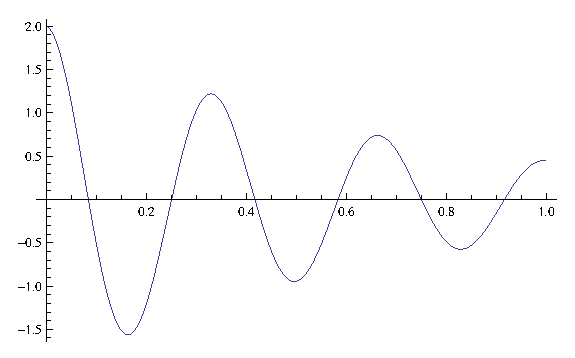
\includegraphics{exercise17.eps}

          Exercise 17: $f(t) = 2 e^{-1.5t} \cos 6 \pi t$
        \end{figure}

      \item[18]
        \begin{figure}[H]
          \centering
          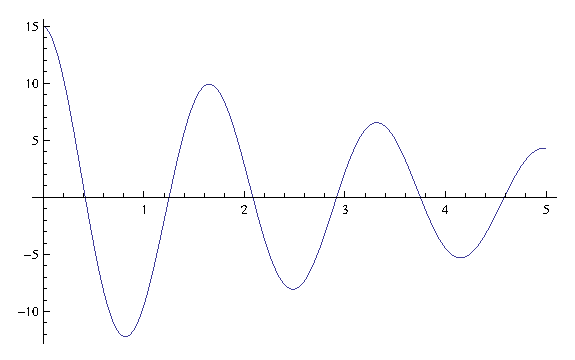
\includegraphics{exercise18.eps}

          Exercise 18: $f(t) = 15 e^{-0.25t} \cos 1.2 \pi t$
        \end{figure}

      \item[19]
        \begin{figure}[H]
          \centering
          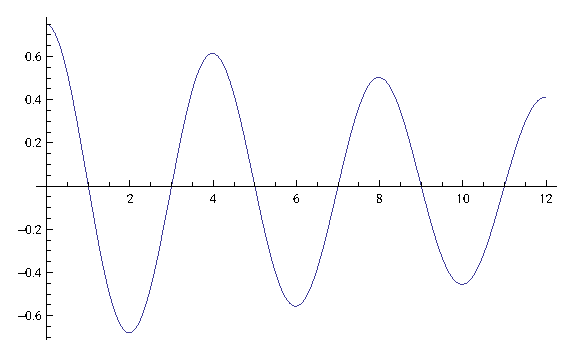
\includegraphics{exercise19.eps}

          Exercise 19: $f(t) = 100 e^{-0.05t} \cos \frac{\pi}{2} t$
        \end{figure}

      \item[25]
        \pagebreak

        \begin{enumerate}[(a)]
          \item $f = \frac{20 \pi}{2 \pi} = \boxed{ 10 }$

          \item 
            \begin{figure}[H]
              \centering
              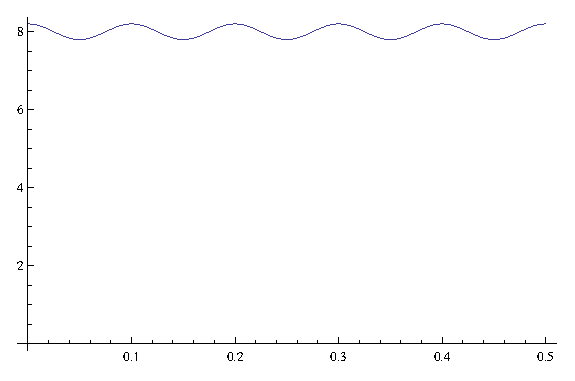
\includegraphics{exercise25.eps}

              Exercise 25
            \end{figure}

          \item $y_{max} = \boxed{ 8.2 }$

        \end{enumerate}

      \item[26]
        \begin{align*}
          \text{period}    & = \frac{2 \pi}{2 \pi (9.15 \times 10^7)} \approx \boxed{ \unit[1.093 \times 10^{-8}]{m} } \\
          \text{frequency} & = \frac{2 \pi (9.15 \times 10^7)}{2 \pi} = \boxed{ \unit[9.15 \times 10^7]{cycles/s} } \\
        \end{align*}

      \item[27]
        \begin{enumerate}[(a)]
          \item $y_{max} = \boxed{ \unit[8900]{animals} }$

          \item The length of time between maximums is the period:
            \[
              \text{period} = \frac{2 \pi}{2} \approx \boxed{ \unit[3.14]{years} } \\
            \]
        \end{enumerate}

      \item[28]
        \pagebreak
        \begin{enumerate}[(a)]
          \item 
            \begin{align*}
              \text{amplitude} & = \boxed{ \unit[25]{mmHg} } \\
              \text{period}    & = \frac{2 \pi}{160 \pi} \approx \boxed{ \unit[0.0125]{minutes/beat} } \\
              \text{frequency} & = \frac{160 \pi}{2 \pi} = \boxed{ \unit[80]{beats/minute} } \\
            \end{align*}

          \item 
            \begin{figure}[H]
              \centering
              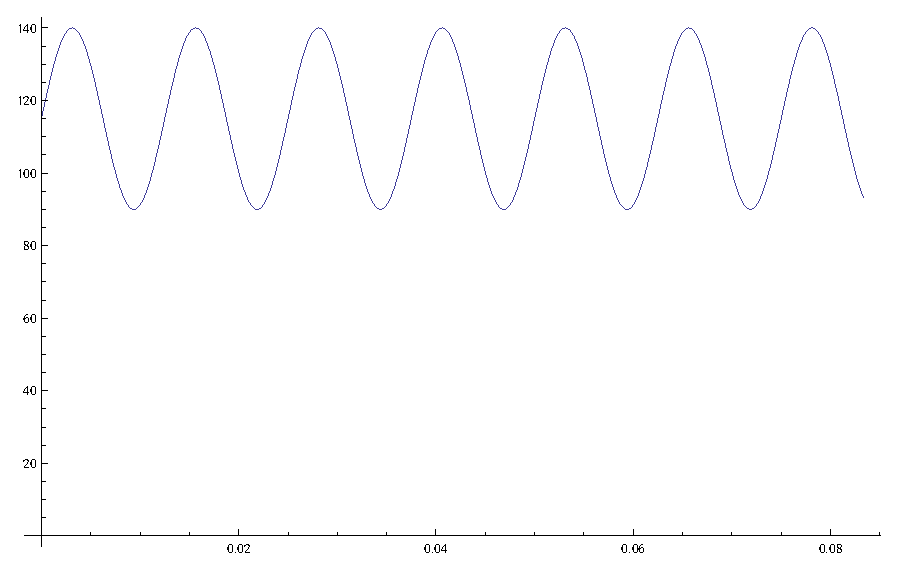
\includegraphics[scale=0.6]{exercise28.eps}

              Exercise 28
            \end{figure}

          \item The period decreases and the frequency increases.

        \end{enumerate}

      \item[29] The period is \sfrac{2}{5} so: 
        \[
        \omega = \frac{2 \pi}{\sfrac{2}{5}} = 5 \pi
        \]

        The amplitude is 5 and the final function is:
        \[
          \boxed{ d(t) = 5 \sin 5 \pi t }
        \]

      \pagebreak

      \item[30] The period is 12 hours so: 
        \[
          \omega = \frac{2 \pi}{12} = \frac{\pi}{6}
        \]

        The amplitude is 6 and the function is an inverted sine, so the final function is:
        \[
          \boxed{ d(t) = -6 \sin \frac{\pi}{6} t }
        \]

      \item[32] The period is 1 second so: 
        \[
          \omega = \frac{2 \pi}{1} = 2 \pi
        \]

        The amplitude is 2 and the spring starts out at a negative position, so the function is:
        \[
          \boxed{ d(t) = -2 \cos 2 \pi t }
        \]

      \item[34]
        \begin{enumerate}[(a)]
          \item $f(t) = 5 \cos \sqrt{\frac{3}{10}} t$

          \item $f = \frac{ \sqrt{\sfrac{k}{m}} }{2 \pi}$

          \item If the mass increases the frequency decreases.

          \item If the spring gets stiffer the frequency increases.

        \end{enumerate}

      \item[35] The period is 20 seconds so: 
        \[
          \omega = \frac{2 \pi}{20} = \frac{\pi}{10}
        \]

        The center of the wheel is at 11, so the function is:
        \[
          \boxed{ h(t) = 11 + 10 \cos \frac{\pi}{10} t }
        \]

      \item[37] The period is 10 days so: 
        \[
          \omega = \frac{2 \pi}{10} = \frac{\pi}{5}
        \]

        The function is:
        \[
          \boxed{ m(t) = 3.8 + 0.2 \cos \frac{\pi}{5} t }
        \]

      \item[39]
        \[
          \omega = 100 \cdot 2 \pi = 200 \pi
        \]

        The function is
        \[
          \boxed{ v(t) = 310 \cos 200 \pi t }
        \]

        The rms voltage is: $\frac{310}{\sqrt{2}} \approx \boxed{ \unit[ 220 ]{ volt } }$ 

      \item[40]
        \[
          \omega = \frac{2 \pi}{24} = \frac{\pi}{12}
        \]

        Since the pressure varies by $\pm 20$, the amplitude is $20$.

        The maximum occurs 14 hours after midnight, so the phase shift is 14 hours.

        The function is
        \[
          \boxed{ p(t) = 100 + 20 \cos \frac{\pi}{12} (t - 14) }
        \]

      \item[41]
        \begin{enumerate}[(a)]
          \item $\boxed{ v_{max} = 45 }$

          \item The generator completes 4 cycles in 0.1 seconds, so the frequency is $\boxed{ \unit[ 40 ]{cps} }$

          \item The armature is rotating at $\boxed{ \unit[ 40 ]{rpm} }$

          \item $\boxed{ v(t) = 45 \cos 80 \pi t }$

        \end{enumerate}

      \pagebreak

      \item[42]
        \begin{enumerate}[(a)]
          \item 
            \begin{itemize*}

              \item moving towards: 
                \begin{align*}
                  f & = 500 \cdot \frac{1130}{1130 - 110} \\
                    & \approx \boxed{ \unit[554]{Hz} } \\
                \end{align*}

              \item moving away: 
                \begin{align*}
                  f & = 500 \cdot \frac{1130}{1130 + 110} \\
                    & \approx \boxed{ \unit[456]{Hz} } \\
                \end{align*}

            \end{itemize*}

          \item 
            \begin{itemize*}
              \item moving towards: 
                \begin{align*}
                  f(t) & = A \sin 554 \cdot 2 \pi t \\
                       & = \boxed{ A \sin 1108 \pi t } \\
                \end{align*}
              \item moving away: 
                \begin{align*}
                  f(t) & = A \sin 456 \cdot 2 \pi t \\
                       & = \boxed{ A \sin 912 \pi t } \\
                \end{align*}
            \end{itemize*}
        \end{enumerate}

      \item[44]
        \begin{align*}
          e^{-3c} & = 0.25 \\
          -3c     & = \ln 0.25 \\
          c       & = - \frac{\ln 0.25}{3} \\
                  & \approx \boxed{ 0.4621 } \\
        \end{align*}

      \pagebreak

      \item[46]
        \begin{enumerate}[(a)]
          \item 
            First find by what factor the amplitude has decreased:
            \begin{align*}
              0.6 & = x \cdot 3 \\
              x   & = 0.2 \\
            \end{align*}

            now find the damping factor:
            \begin{align*}
              e^{-2c} & = 0.2 \\
              -2c     & = \ln 0.2 \\
              c       & = - \frac{\ln 0.2}{2} \\
                      & \approx \boxed{ 0.8047 } \\
            \end{align*}

          \item 
            \begin{align*}
              f(t) & = e^{-0.8047t} 3 \cos 165 \cdot 2 \pi \\
                   & = \boxed{ e^{-0.8047t} 3 \cos 330 \pi } \\
            \end{align*}

        \end{enumerate}

    \end{description}

  \else
    \vspace{10 cm}
    \begin{quote}
      \begin{em}
        Your vision will become clear only when you look into your heart \dots Who looks outside, dreams. Who looks inside, awakens.
      \end{em}
    \end{quote}
    \hspace{1 cm} --Carl Jung
  \fi

\end{document}

